\chapter{The unforgiving LOS-state}\label{ch:deepindoor}
The task of predicting attenuation of radio transmission in \gls{o2o} scenarios increases in complexity with increased distance, due to the increased number of objects in the radio environment. The task of predicting attenuation in \gls{o2i} is significantly more complex, due to specific interactions of the different materials in between the transmitter and receiver antennas. The campus of The Technical University of Denmark (DTU) consists of a unique underground system. Given the efforts spent in understanding and applying Deep Learning to path loss estimation for \gls{o2o} scenarios, utilizing this unique tunnel system for studies seemed relevant for improving and evaluating current models available in the literature. The results are formalized into two publications

\begin{itemize}
    \item \textbf{Investigation of deep indoor NB-IoT propagation attenuation}, IEEE VTC-Fall 2019 \cite{Malarski2019InvestigationAttenuation}
    \item \textbf{Experimental Evaluation of Empirical NB-IoT Propagation Modelling in a Deep-Indoor Scenario}, submitted for Globecom 2020 \cite{Thrane2020ExperimentalScenario}
\end{itemize}

The former introducing the concepts of Deep Indoor propagation modelling with an initial measurement study. This was extended in the latter work, with an extensive measurement campaign utilizing complex LIDAR data to offer accurate positions and features. The latter is furthermore the foundation for the majority of the content throughout this chapter. 

\section{Deep Indoor}

With the development and standardization of \gls{lpwan} technologies such as \gls{nbiot} battery-powered sensors are being deployed in unreachable scenarios (usually indoor) to allow for new application and services \cite{Sinha2017ANB-IoT}. New applications will result in a significant number of complex deployment situations where accurate coverage and capacity estimation is a necessity \cite{Lauridsen2016CoverageArea, Vejlgaard2017}. Current deployments of \gls{nbiot} sites commonly takes place outdoor. In this case, the transmission to \glspl{ue} inside buildings or structures is termed \gls{o2i}. A comprehensive introduction and summary of the inner workings and best practices for deploying \gls{nbiot} can be found in references such as \cite{Sinha2017ANB-IoT, Li2018SmartNB-IoT, Chen2017NarrowThings} and references herein.

The applications of \gls{nbiot} are many due to the long-range transmission properties, and the battery-operated sensors. The use of \gls{nbiot} to remote monitoring is subject to reliability concerns regarding 1) reliably connectivity and 2) regulated power consumption. For instance, placing sensors in hard to reach areas, such as used for smart water metering the sensors must be reliable and not subject to repair or replacement within short periods of deployment \cite{Popli2019AChallenges}. 



\begin{figure*}
    \centering
    
\includegraphics{chapters/part_pathloss/figures/outdoor_to_indoor/approach_figure.eps}
    \caption{Deployment of sensors in deep indoor situations may require displacement or added relays to ensure the desired connection reliability.}
    \label{fig:outdoor_to_indoor_approach}
\end{figure*}

Coverage and capacity modelling is an essential element for deploying any \gls{nbiot} sensor, and an even more critical aspect when deploying sensors in hard to reach areas, especially from the perspective of the \gls{mno}, but also the consumer and enterprise developing the sensors. For instance, as visualized in Fig. \ref{fig:outdoor_to_indoor_approach} some sensors might require displacement to ensure a reliable connection, and in some cases, it might even be necessary to deploy local relays offering \gls{i2i} propagation. Both of which require expensive trial-and-error experiments if no accurate coverage modelling can be applied.  

\subsection{Outdoor-To-Indoor empirical models}
Both \gls{3gpp} and \gls{itu} have in the latest technical reports, concerning coverage models and path loss estimation, supplied with so-called \gls{o2i} models. The models provide with terms for attenuation associated with 1) penetration losses and 2) the distance inside the building. The documents are focused on indoor scenarios related to regular buildings. E.g. distances indoor define the distance to the outermost wall that separates the receiver antenna from the transmitter antenna. More specifically, the losses are composed as followings

\begin{equation}\label{eq:o2i_pl}
    PL_{O2I} = PL_{b} + PL_{tw} + PL_{in}
\end{equation}

Where $PL_{b}$ is the basic outdoor path loss as denoted by the \uma{A} and \uma{B} models as described in Section \ref{sec:empirical_path_loss}. The terms, $PL_{tw}$ and $PL_{in}$ are losses associated with building penetration and the distance indoor respectively. The losses associated with the penetration, are composed into a low-loss and high-loss model, both being frequency-dependent, but constant with distance.  On the other hand, losses related to indoor distance ($PL_{in}$) are dependent on an indoor distance parameter as follows.

\begin{equation}\label{eq:o2i_pl_in}
    PL_{in} = 0.5 \cdot d_{in,2d}
\end{equation}

Where $d_{in,2d}$ denotes the distance indoor, i.e. the distance to the outermost wall in the direction of the transmitter. The entirety of Eq. (\ref{eq:o2i_pl}) are undefined for indoor scenarios different from level 0, 1 and 2. Furthermore, the indoor distance metrics are unspecified for underground positions. 

The remainder of this chapter contains an experimental investigation for deep indoor path loss modelling. More specifically, evaluating current models and the performance for scenarios that are different than regular buildings, i.e. \gls{o2i} where the indoor attenuation is partially underground. 

\subsection{Deep Indoor attenuation}
Radio propagation modelling for tunnels has been subject to significant research due to the many radio applications residing in tunnels. For instance, railway operators require reliable communication networks to ensure safety and effective maintenance. A comprehensive survey of radio propagation modelling for tunnels can be found in \cite{Hrovat2014ATunnels}. The paper discusses the use of ray-tracing models and empirical models (among others) and the resulting predictive accuracy. It is found that the geometry of the tunnel system, especially the cross-sectional shape, is significantly essential for estimation of radio propagation. It is found that ray-tracing models that utilize such cross-sectional geometry information perform better in both NLOS and LOS situations. However, this is not the case for empirical models that are found to be lacklustre in predictive performance when predicting the NLOS state. Finally, it should be said that the scope of the research generally considers transmission within tunnel systems. In other words, the unreliable transmission characteristics of \gls{o2i} push \acrlong{mno} to install relays and base stations inside the tunnel systems making radio propagation models inside tunnels relevant. The purpose of the study is not to enrich literature with improved empirical models for radio propagation in tunnel systems. It is, however, the objective to investigate how current empirical models perform for \gls{nbiot} technologies in a \gls{o2i} transmission scenario.

\section{Deep Indoor Measurements}
Getting positions indoor is not a trivial task, as common solutions using \gls{gnss} are unavailable. Techniques for inferring positions indoor using radio waves with high accuracy have been documented in literature \cite{Nuaimi2011}. However, such solutions require complicated infrastructure and post-processing. In this particular case, the unique tunnel system is scanned using high-resolution LIDAR. The availability of such data enables accurate indoor positioning and advanced feature engineering for investigating indoor attenuation and parameters related hereof.  Initial evaluations of deep indoor attenuation were completed in \cite{Malarski2019InvestigationAttenuation}, using a simplistic metric of indoor distance. It shows an inaccuracy of using $PL_{in}$ in deep indoor scenarios but is subject to additional measurements and research. The availability of the LIDAR data increases the accuracy of the study and the resulting indoor distance features. 


\subsection{Tunnel system}
The tunnels span the entirety of the Technical University of Denmark campus, providing a unique location for long-distance deep indoor measurements. The layout and measurements conducted are visualized in Fig. \ref{fig:underground_tunnel_system}.

\begin{figure}
    \centering
    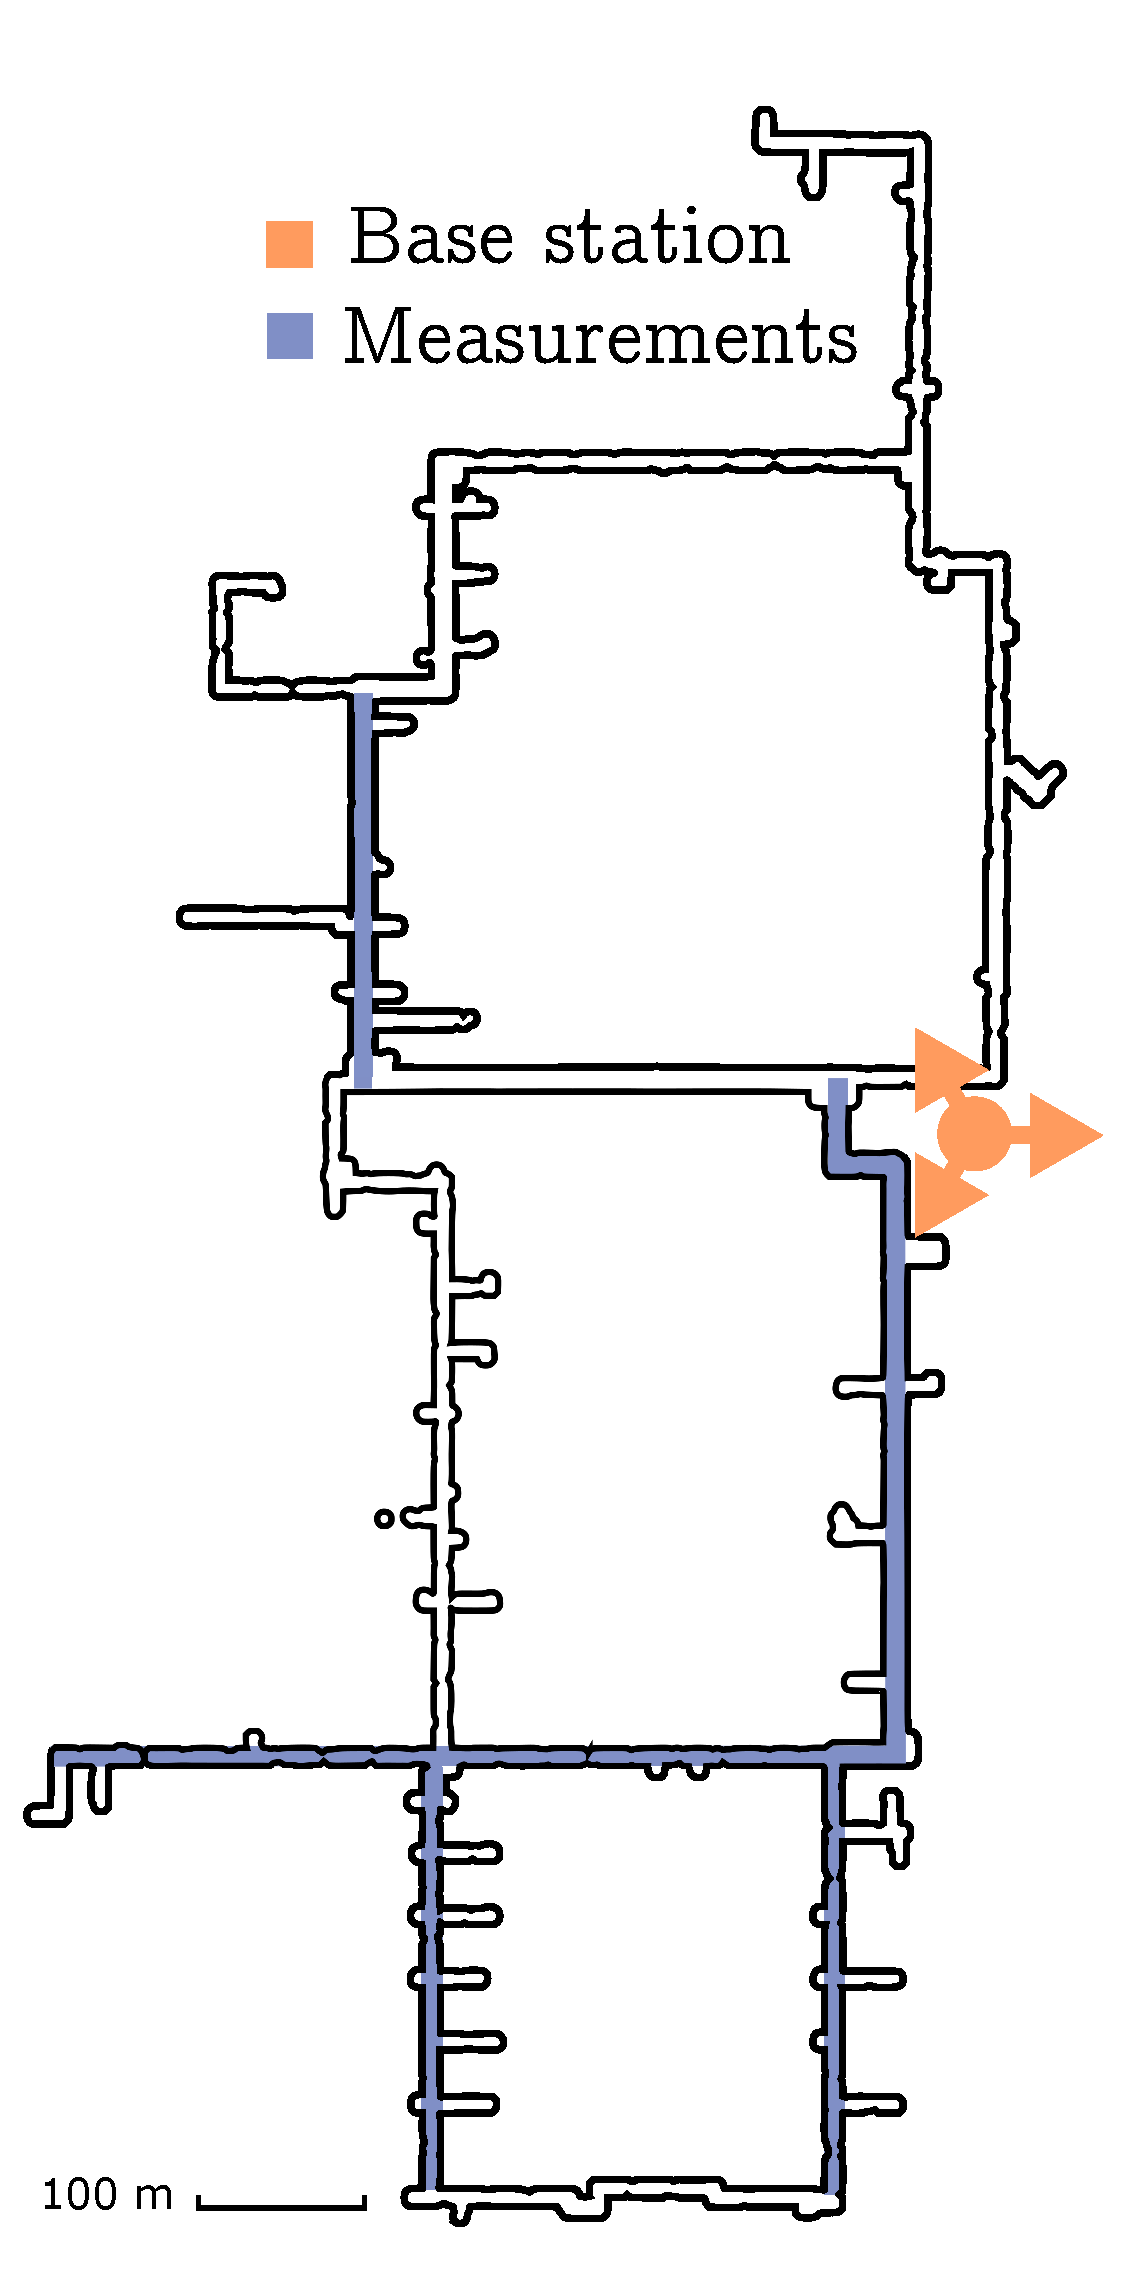
\includegraphics[width=0.5\textwidth]{chapters/part_pathloss/figures/outdoor_to_indoor/Complete_tunnel_system.eps}
    \caption{The underground tunnels of The Technical University of Denmark campus. The areas of measurements are highlighted.}
    \label{fig:underground_tunnel_system}
\end{figure}





\subsection{LIDAR}
A complete LIDAR scan of the tunnel system has been conducted with a very granular resolution of $> 1$ cm. The LIDAR data provides with a set of $3$D coordinates $(x_i, y_i, z_i)$ for the entirety of the tunnel system, accumulating to $\approx 20$ GB of files, with approximately $100$ million coordinate pairs. Custom LIDAR scripts have been written to process the data. The was largely enabled by libraries such as LasPy \cite{Grantbrown/laspy:1.0-1.4.} for LIDAR file processing, and \cite{alan_d_snow_2020_3714221} for coordinate conversion. Examples of the point cloud and the data can be seen in Fig. \ref{fig:tunnel_cross_section} and Fig. \ref{fig:tunnel_3d_view}.

\begin{figure*}
    \centering
    \caption{Cross-sections of a tunnel corridor on the xz-plane. Details of pipes, ventilation and other indoor features are visible.}\label{fig:tunnel_cross_section}
    \subfloat[]{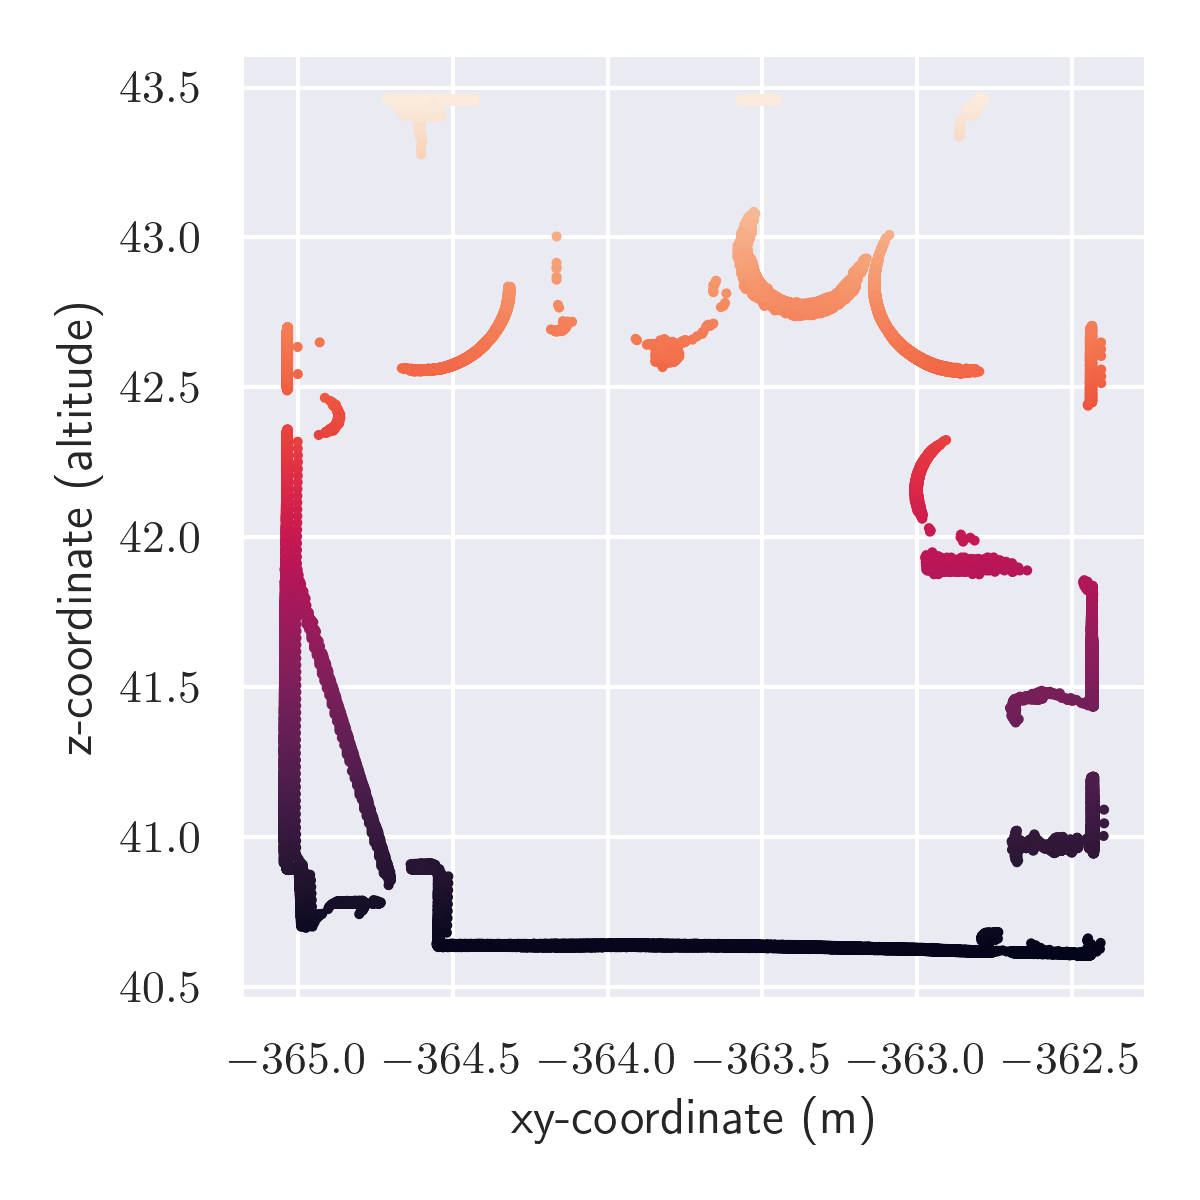
\includegraphics[width=0.3\textwidth]{chapters/part_pathloss/figures/outdoor_to_indoor/crossection_1.png}}
    \subfloat[]{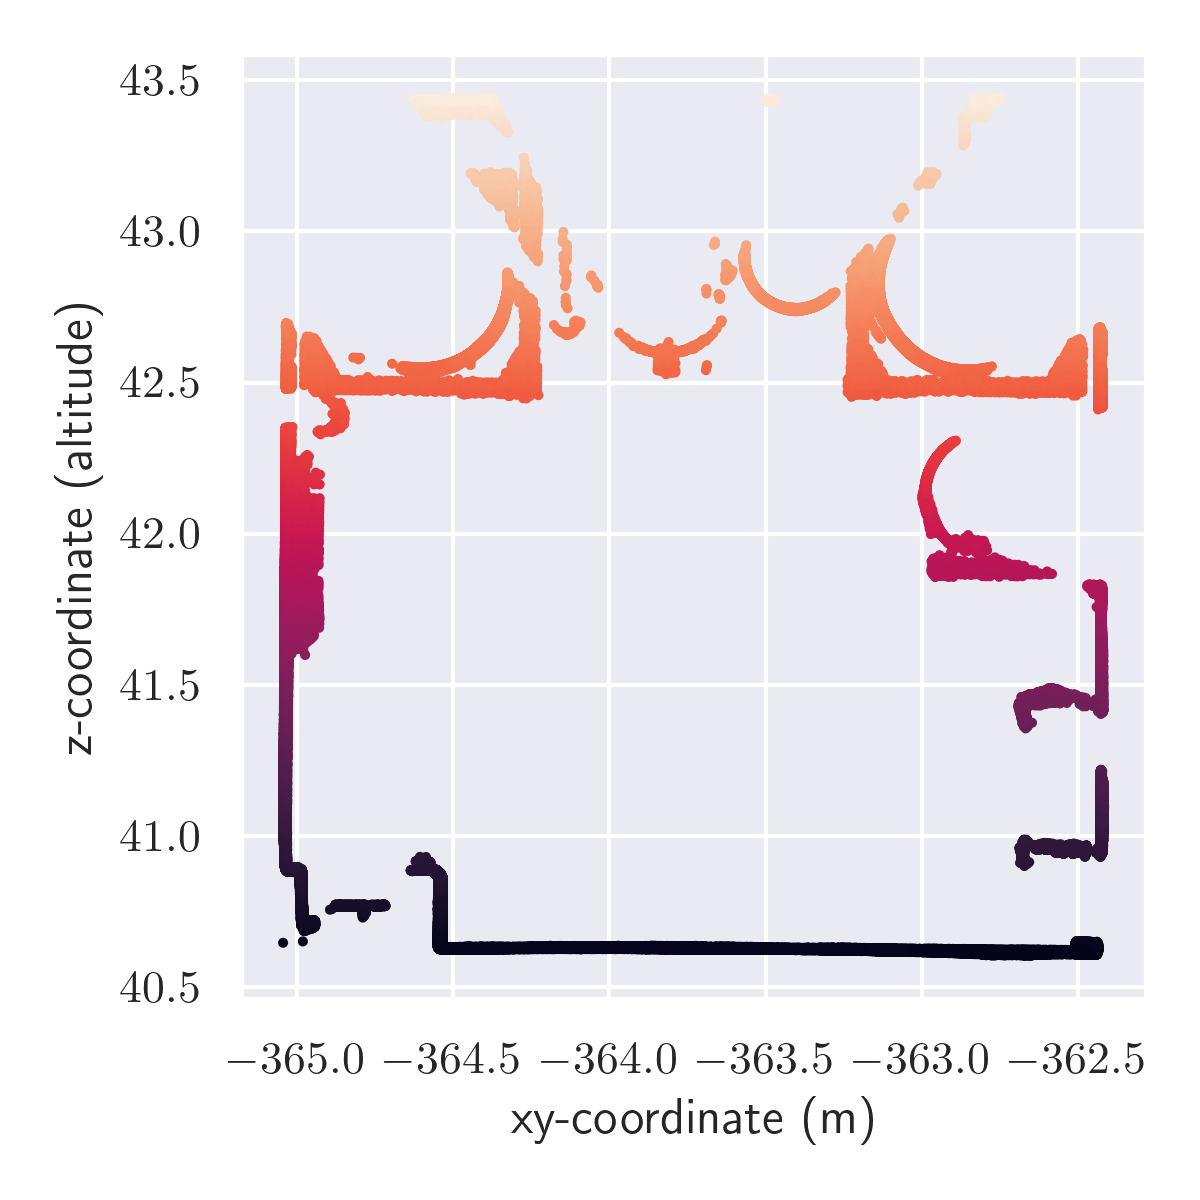
\includegraphics[width=0.3\textwidth]{chapters/part_pathloss/figures/outdoor_to_indoor/crossection_2.png}}
    \subfloat[]{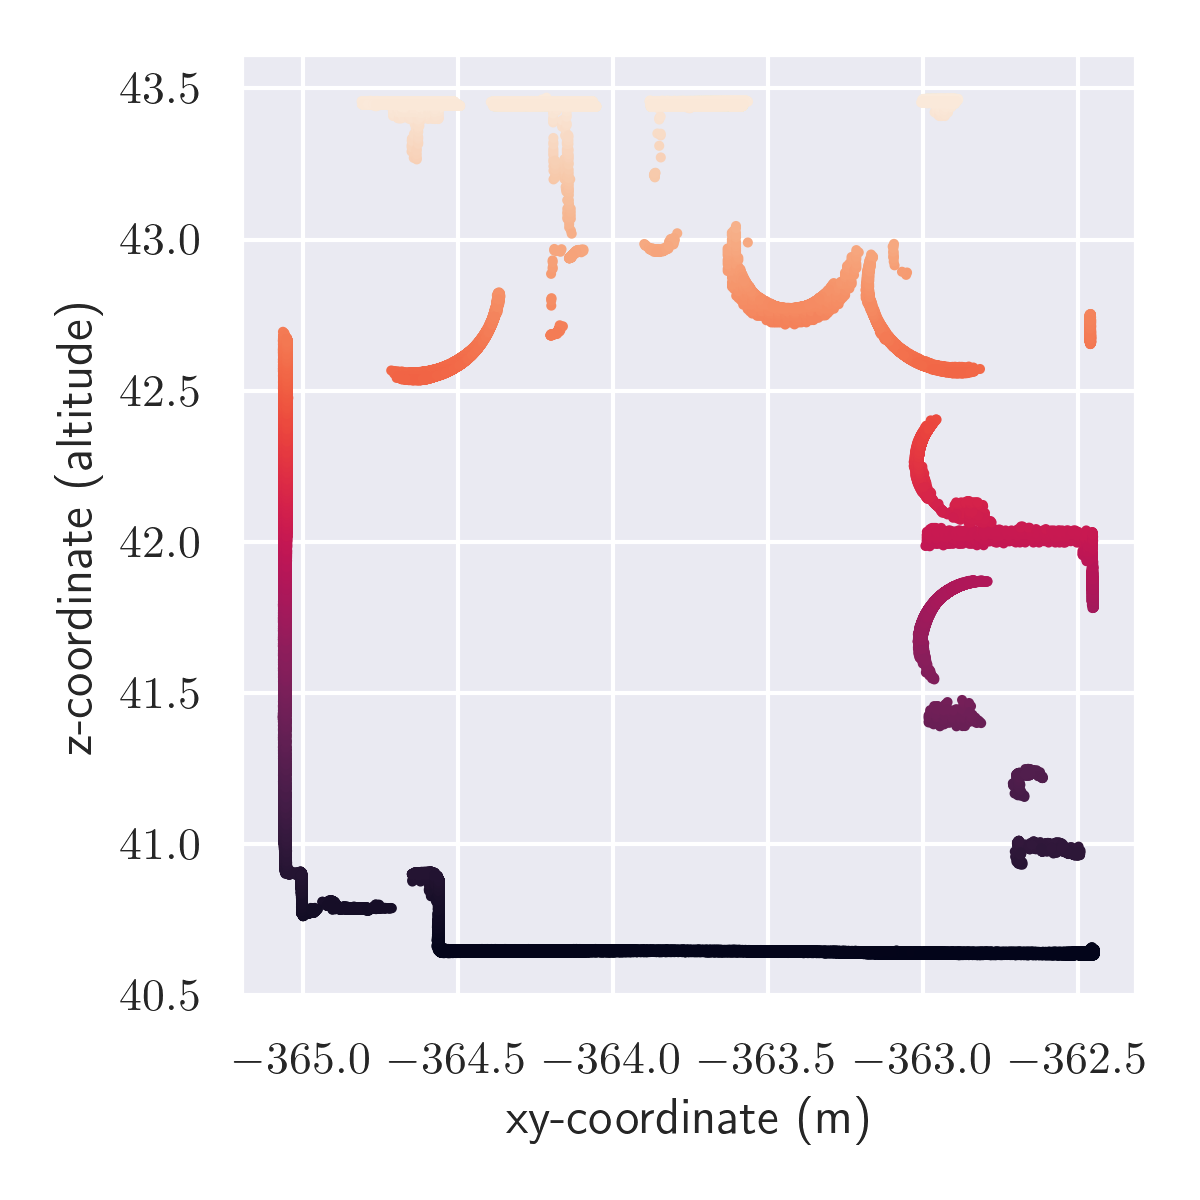
\includegraphics[width=0.3\textwidth]{chapters/part_pathloss/figures/outdoor_to_indoor/crossection_3.png}}
    \vspace{2em}
\end{figure*}

The LIDAR coordinate pairs are given in a coordinate system related to that of the DTU campus termed DTULOK. A procedure for converting to the UTM32 system is supplied along with the dataset, consisting of a so-called Helmert transformation. 


\begin{figure}
    \centering
    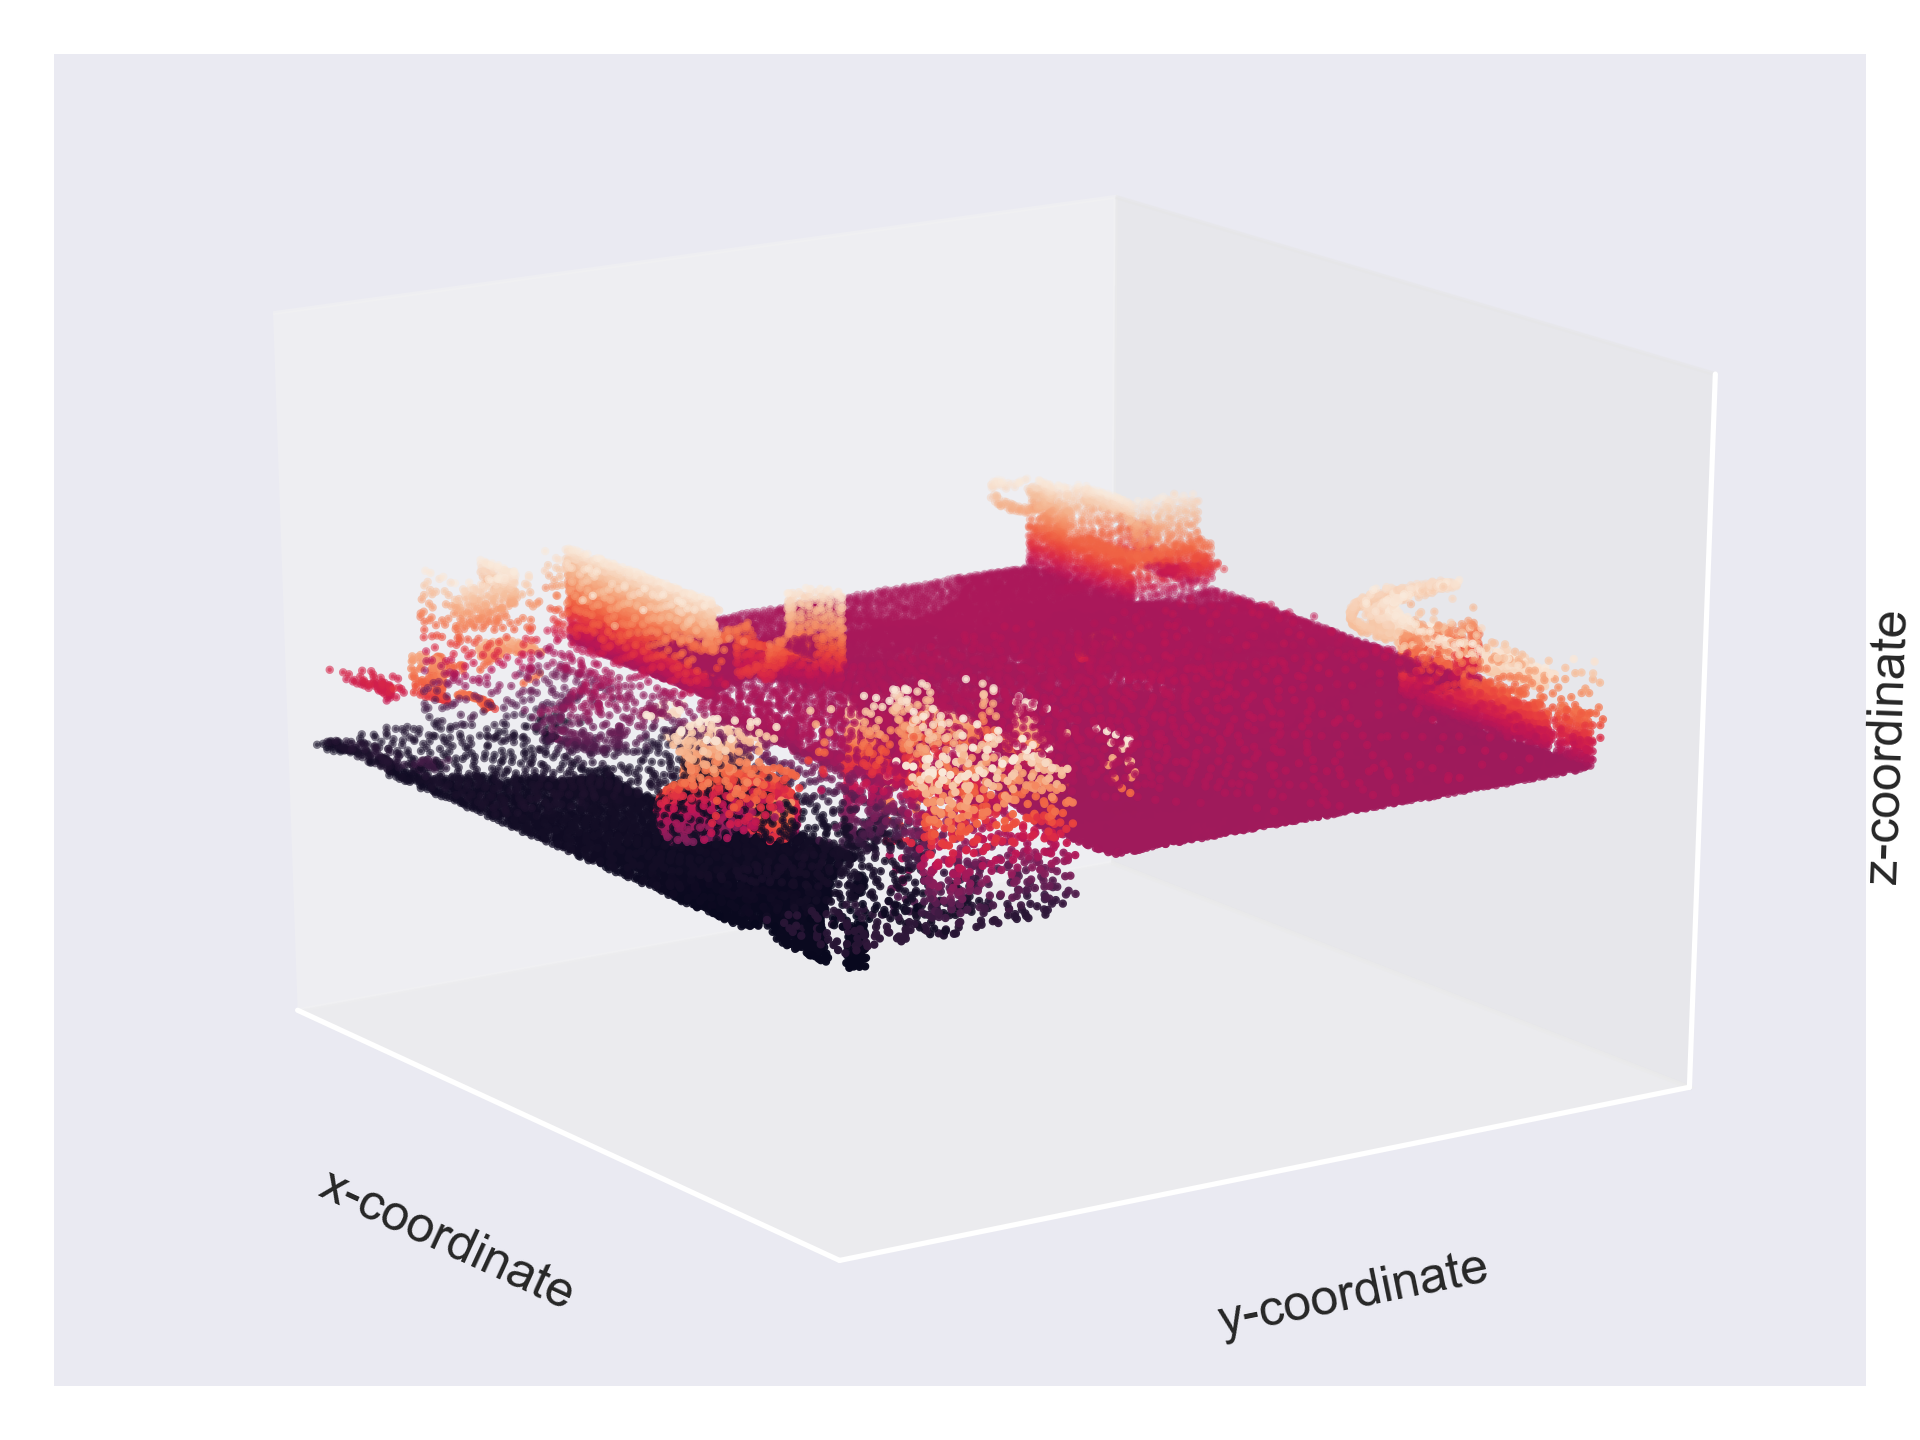
\includegraphics[width=\textwidth]{chapters/part_pathloss/figures/outdoor_to_indoor/3d_view.png}
    \caption{$3$D view of the LIDAR pointcloud limited on the Z-axis to show a horizontal cross-section.}
    \label{fig:tunnel_3d_view}
\end{figure}


\subsection{Setup}

\begin{table}[htbp]
\centering
\begin{tabular}{@{}l|l@{}}
\toprule
\# of measurement points       & $895$             \\ \midrule
TSMW/UE measurements per point & $1e6/10$          \\ \midrule
Operating frequency            & $820.5$ MHz       \\ \midrule
Bandwidth                      & $180$ kHz         \\ \midrule
Noise figure (TX/RX)           & $5$ dB/$3$ dB     \\ \midrule
TX power                       & $46$ dBm          \\ \midrule
Receiver antenna position      & Vertical          \\ \midrule
TX/RX antenna gain             & $5$ dBi/$5.8$ dBi \\ \bottomrule
\end{tabular}
\caption{Measurement configuration and parameters}\label{tab:measurement_configuration}
\end{table}

The setup consists of a \gls{r_and_s} TSMW Network Tester \cite{Manual2017} (as also utilized for drive-testing, see Appendix \ref{app:drive_test_study_2017} and \ref{app_drive_test_study_2020}). And a \gls{nbiot} device \cite{sodaq}. Antennas for both the TSMW, and the \gls{nbiot} device was mounted vertically on a trolley. Utilizing a laptop with a set of parallel measurement scripts, measurements from both the TSMW and \gls{nbiot} device were conducted for each measurement position. More specifically, a measurement was taken with constant intervals for individual corridors. This results in $N$ measurements for each corridor, ideally equidistant spaced with $1$ to $2$ m. For each decided measurement position, the following measurements were taken

\begin{itemize}
    \item $1e6$ \gls{iq} samples (TSMW)
    \item $10$ \gls{rsrp} Measurements distributed over $20$ seconds (\gls{nbiot} device)
\end{itemize}


The \gls{iq} samples were taken utilizing a low-pass filter centred around the \gls{nbiot} operating carrier frequency given the bandwidth of a single narrowband of $180$ kHz. An overview can be found in Table \ref{tab:measurement_configuration}. 

The \gls{rsrp} measured was averaged over all samples taken at each measurement position to average out any time-variant impairments that may have influenced the \gls{rsrp} at time of measurements. 


\subsection{Indoor positioning}
A method was developed for inferring indoor positioning from the LIDAR scan. It can be summarized as the following step-wise procedure. It consists of the following steps:

\begin{enumerate}
    \item Identify start and end positions of measurement campaigns within the $3$D point cloud.
    \item Interpolate measurement positions ($x, y$) given the start and end positions and the number $N$ measurements conducted.
    \item Look-up the interpolated coordinates to obtain ($x, y, z$) pairs.
    \item Convert local coordinate system (DTULOK) to UTM32/WSG84
\end{enumerate}

Accurate identification of the start and end positions within the point cloud (step 1) is paramount to high accuracy for the remainder of the measurement positions. The step was split into two procedures for achieving accurate identification, a) ensuring the start and end positions were well documented with pictures and can visually be identified using, e.g. a large pipe or other significant characteristics of the environment. b) an interactive program was created to narrow down such characteristics within the point cloud. An example can be seen in Fig. \ref{fig:tunnel_3d_view}. 

The interpolation (step 2) assumes equidistant measurements. It is fair to expect some errors may introduce themselves during the measurements, however, by ensuring the total distance between the start and end position is divided into $N$ segments, the overall equidistant error is averaged out.

The look-up of coordinates (step 3) consisted of computing the distance (euclidean) to LIDAR coordinate pairs. The closest point within the point cloud was then extracted as the coordinate. Due to the high resolution, on average, the nearest data point was within a margin of $1$ cm.

The LIDAR data operates within a coordinate system localized to the area of measurements. A conversion (step 4)  to more generic coordinate systems such as UTM32 and WSG84 (Latitude, Longitude) \cite{alan_d_snow_2020_3714221} completed the indoor positioning procedure. 

%% Here

\section{Evaluation of indoor KPIs}
The literature for indoor attenuation states that 1) tunnel geometry is considered the main influence on attenuation for propagation in tunnels, and 2) current models for \gls{o2i} use a simple indoor distance metric. Having access to the high resolution LIDAR data enables the engineering for indoor distance metrics with high accuracy. 


\subsection{Feature Engineering}
The bearing between the receiving and transmitting antenna (also known as the azimuth angle $\phi$) can be determined by the WGS$84$ coordinates of the measurement position and the transmitting antenna. Additionally, the altitude information provided by the LIDAR data, offers means for computing the elevation angles (the height of the transmitter is known). Thus, the accurate indoor position in $3$D enables simple computation of the azimuth ($\phi$) and elevation ($\theta$) angles. Furthermore, this in combination with the LIDAR data enables distance calculations in both $2$D and $3$D space. 

In order to be capable of computing the require indoor distance metrics, a few requirements are needed. Firstly, the tunnel geometry must be quantified such that distances can be computed to intersecting tunnel walls and edges. Secondly, height of the terrain must be know, at points in space where the "straight-as-the-crow-flies" path to and from the transmitting antenna intersects with the terrain. Formalizing the tunnel geometry was done by inspecting the LIDAR data and designing so-called boundary boxes in $3$D space. Thus, the boundary boxes determine the geometry of the measured tunnel for a given set of measurements. By doing so, and applying trigonometry, the following set of distance metrics in $3$D space was derived.

\begin{itemize}
    \item Indoor distance to the intersecting tunnel wall/edge $d_{in}$.
    \item Penetration distance, distance between the tunnel wall/edge and the terrain $d_{pen}$.
    \item Average $2$D distance to intersecting corridor $d_{cor,avg}$
\end{itemize}


\begin{figure}
    \centering
    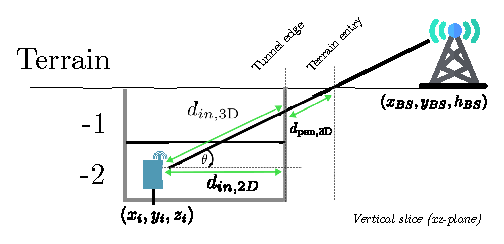
\includegraphics{chapters/part_pathloss/figures/outdoor_to_indoor/inside_distance_illustration.eps}
    \caption{Distance metrics utilizing tunnel geometry and accurate indoor positions using elevation angles $\theta$}
    \label{fig:inside_distance_xz}
\end{figure}

\begin{figure}
    \centering
    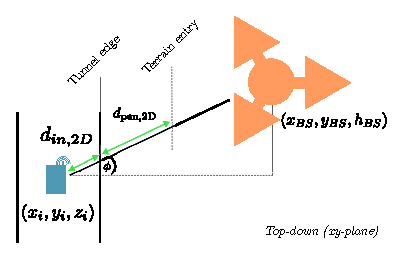
\includegraphics{chapters/part_pathloss/figures/outdoor_to_indoor/inside_distance_illustration_xyplane.eps}
    \caption{Distance metrics utilizing tunnel geometry and accurate indoor positions using azimuth angles $\phi$}
    \label{fig:inside_distance_xy}
\end{figure}

\noindent A few edge cases arose when using the engineered boundary boxes of the tunnel geometry. Firstly, a set of measurements were almost directly below that of the transmitter (as seen by Fig. \ref{fig:underground_tunnel_system}). This resulted in a set of elevation angles, where the tunnel edge/wall was not the correct intersection between the "straight-as-the-crow-flies" path and the tunnel geometry. Instead, the roofing of the tunnel was the \emph{entry} point of the direct path. This required a re-computation of the distance metrics using a more advanced $3$D trigonometry approach. 

Secondly, some parts of the corridors consisted of several intersecting corridors. This meant that the distance to the tunnel edge/wall became dependent on a non-rectangular boundary box covering the tunnel measured. Such a boundary box is time-consuming and exhaustive to create in $3$D space. However, by doing so the engineering of the feature $d_{cor,avg}$ was enabled using unique identifers for each intersecting tunnel across the system.

Finally, the terrain information for computing and deriving the penetration distance did not include any buildings. A so-called \gls{dtm} \cite{kortforsyningen} was utilized for extracting altitude information, effectively providing an accurate approximation of the terrain covering the area of the underground tunnel system.


\subsection{Results}

\begin{table}
    \centering
    \begin{tabular}{@{}l|ll@{}}
    \toprule
    Regressors               & $R^2$ & Residual MSE \\ \midrule
    $3$D distance              & $0.285$ & $74.973$       \\
    $d_{in,2D}$              & $\mathbf{0.026}$ & $\mathbf{102.098}$      \\
    $d_{in,3D}$              & $0.026$ & $102.097$      \\
    $d_{pen,3D}$             & $0.017$ & $103.022$      \\
    $d_{pen,3D} + d_{in,2D}$ & $0.005$ & $104.335$      \\
    $d_{cor,avg}$            & $\mathbf{0.148}$ & $\mathbf{89.286}$       \\
    $d_{pen,3D} + d_{in,2D}+d_{cor,avg}$ & $0.150$ & $89.276$       \\
    $d_{pen,3D} + d_{in,3D}+d_{cor,avg}$ & $0.150$ & $89.276$       \\
    $\phi + \theta$          & $\mathbf{0.173}$ & $\mathbf{86.763}$       \\ \bottomrule
    \end{tabular}
    \caption{Results of linear regression using OLS \cite{seabold2010statsmodels}}\label{tab:ols_results}
    \vspace{1em}
\end{table}
\noindent The measured \gls{rsrp} concatenated for all measurement subsets (i.e. corridors) are seen in Fig. \ref{fig:indoor_distance_reg} as a function of the $3$D distance (a), and $d_{in,2d}$ (b). Also shown is the prediction of the basic path loss offered by the \gls{3gpp} \gls{uma} model as given by partly by Eq. (\ref{eq:uma_nlos_pathloss_max}). The full path loss model can be found in \cite{38211}. Several (easy separately) clusters are observed for \gls{rsrp} as a function of $d_{in,2d}$, as seen in Fig. \ref{fig:indoor_distance_reg}(b), corresponding to each of the different corridors in which measurements were conducted.

\begin{figure}
    \centering

    \subfloat[Theoretical path loss model vs \gls{rsrp} measurements]{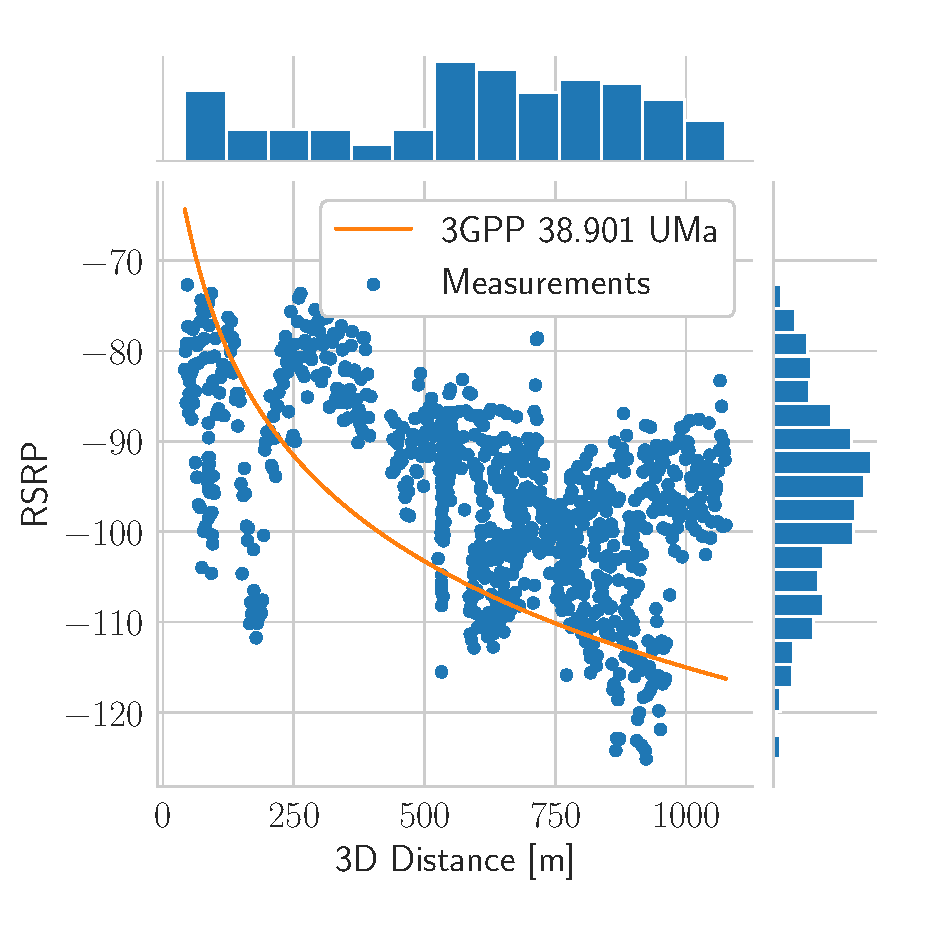
\includegraphics[width=0.8\textwidth]{chapters/part_pathloss/figures/outdoor_to_indoor/results/d3d_rsrp_3gpp.eps}}
    \\
    \subfloat[Indoor distance]{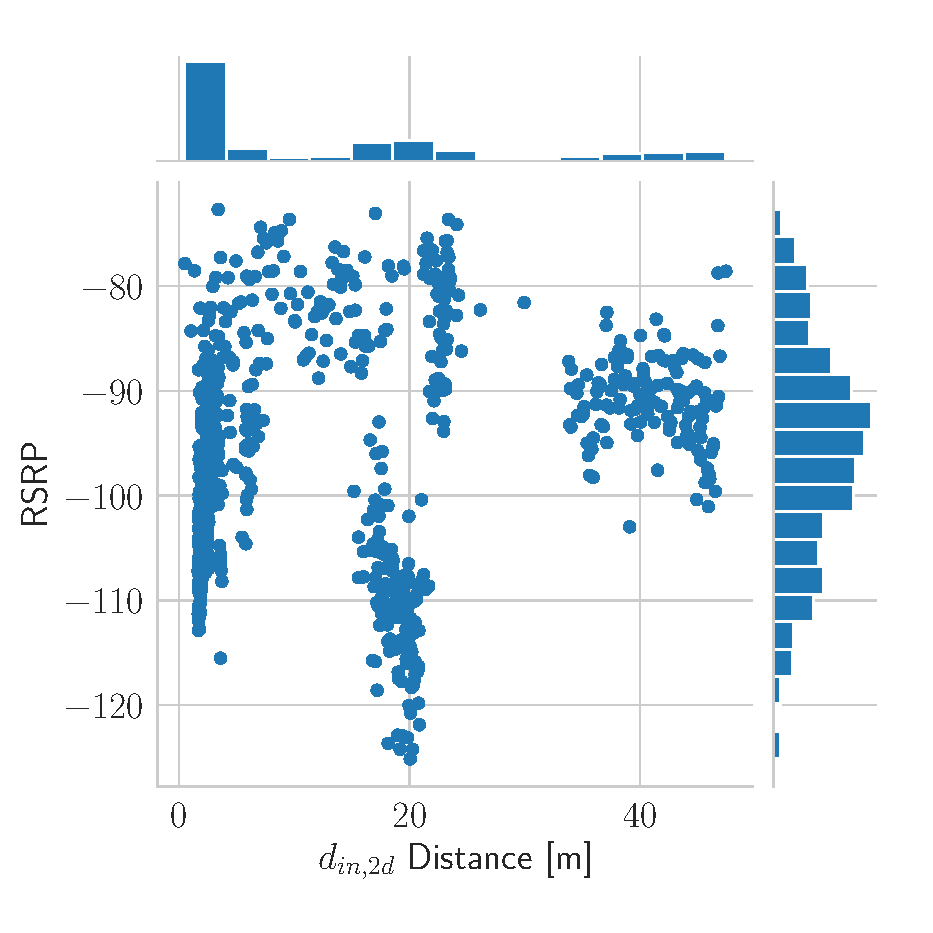
\includegraphics[width=0.8\textwidth]{chapters/part_pathloss/figures/outdoor_to_indoor/results/d2d_wall_rsrp.eps}}
    
    \caption{The prediction provided by the theoretical path loss model $PL_b$ in Eq. (\ref{eq:o2i_pl}) is shown in (a). The indoor distance for all measurements in shown in (b).}\label{fig:indoor_distance_reg}

\end{figure}

The results of a linear regression using \gls{ols} are observed in Table. \ref{tab:ols_results}. The inner workings of the \gls{ols} method are further described in \cite{seabold2010statsmodels}. Briefly summarized it consists of minimizing the sum-of-squares (as is given by Eq. (\ref{eq:sum-of-squares}) using a simple linear model formulation of roughly $y=ax+b$ with the objective to find $a$ and $b$ (a more refined definition can be found in \cite{M.Bishop2006}). 

The results of the linear regression shows a correlation coefficient $R^2$ of $0.026$, with a residual \gls{mse} of $102.098$ using the indoor distance metric of $d_{in,2d}$. Adding and using the elevation angle to obtain $d_{in,3d}$ offers no increase or decrease in the linear model performance. The use of $d_{pen}$ in $3$D have a decrease in  $R^2$ of $\approx 0.001$ compared to the metric of $d_{in}$, and an increase in the residual \gls{mse} of $\approx 1$ dB. Most noticeably is the increase in linear predictive performance when using the parameter $d_{cor,avg}$, and furthermore when utilizing the azimuth and elevation angles $\phi, \theta$.


The predictive performance of utilizing the \gls{o2i} path loss model given by Eq. (\ref{eq:o2i_pl}) is shown in Fig. \ref{fig:mae_boxplot_o2i_pl_in}. The indoor distance parameter of Eq. (\ref{eq:o2i_pl_in}) is altered to use the engineered features of indoor distance, and penetration distance, and a combination of. In other words, the parameter of $d_{in}$ is substituted with the engineered distance features. The \emph{none} case is the use of Eq. (\ref{eq:o2i_pl}) but without the term of $PL_{in}$. It can be seen that the average predictive error of $9.9$ dB is achieved using no terms for attenuation related to indoor distances. A decrease in predictive performance, e.g. an increase in \gls{mae} of $\approx 1.1$ dB is observed utilizing $d_{in,2d}$ as an indoor distance parameter. The performance decreases as the remainder of the engineered features are utilized, peaking at $\approx 26.9$ dB of error using $d_{in,3d}+d_{pen,3d}$ as the indoor distance metric. Finally, it can be said that the performance generally decrease with an increase in distance indoor distance utilizing the proposed model of Eq. (\ref{eq:o2i_pl}).

\begin{figure}
    \centering
    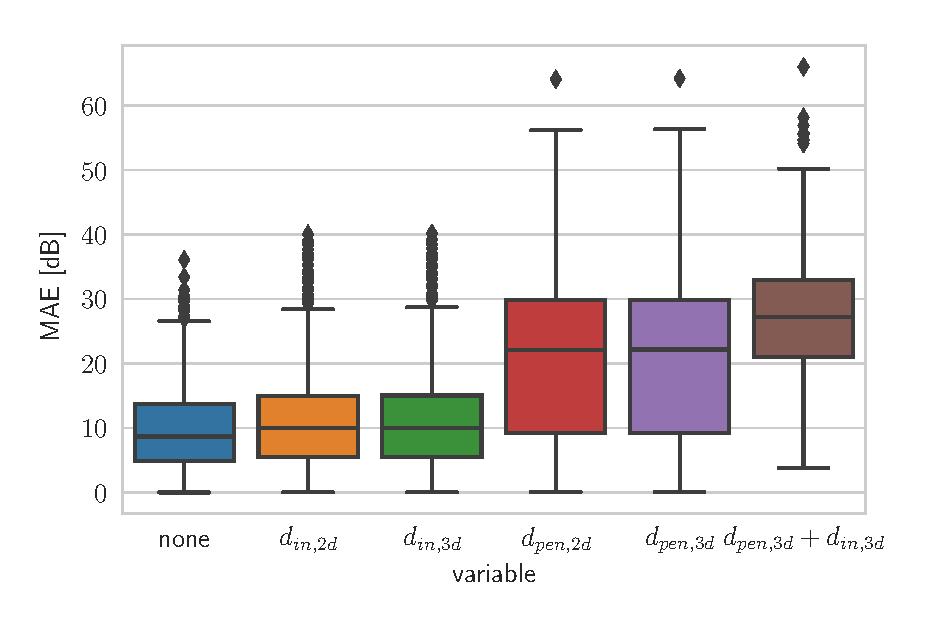
\includegraphics{chapters/part_pathloss/figures/outdoor_to_indoor/results/mae_boxplot.eps}
    \caption{\gls{mae} predictive \gls{rsrp} performance utilizing Eq. (\ref{eq:o2i_pl}) using different indoor distance parameters.}
    \label{fig:mae_boxplot_o2i_pl_in}
\end{figure}

\subsection{Discussion}
The additional path loss based on indoor distance does not in the current state reflect that of Deep-indoor situations. The model of estimating loss associated indoor with indoor distance offer an increase in predictive error of \gls{rsrp} as the indoor distance increase. This is caused by 1) the losses associated with penetration (i.e. $PL_{tw}$) does not reflect the mean attenuation satisfactory, and 2) the model uses a constant term that is distance based. As highlighted by the results of the linear regresssion, using any of the indoor distance metrics of $d_pen$ or $d_in$ is a poor choice of a predictor using a linear model than compared to 1) features of tunnel geometry $d_{cor,avg}$, and 2) angles of azimuth and elevation. From these findings it indicates that A) tunnel geometry-based features are superior to indoor distance features and B) The geo-statistics of the measurement area is complex and thus \gls{rsrp} is highly dependent on local variability. In summary, the findings of A) highlights the importance of tunnel geometry in \gls{o2i} propagation scenarios, and B) Attenuation is largely based on localization, which indicates complex local variability terms.

The engineering of such indoor features of $d_{pen}$ and $d_{in}$ is not a trivial task for underground tunnel systems. Regardless of the features having reduced importance for \gls{rsrp}, obtaining such features is a challenge and is furthermore not suited for use in empirical path loss models. The proposed empirical models should maintain a set of features that are feasible to obtain to motivate the purpose of such models. In this particular case of a tunnel system, the use of any indoor distance metrics to outer wall can be computed using the accurate LIDAR data. However, this is considered a unique data source and is not a common practice in most deep-indoor scenarios. In other words, the attenuation term based on indoor distance provided by Eq. (\ref{eq:o2i_pl_in}) is not only a poor model for tunnel systems, it also requires a feature that in most cases is a challenge to obtain. Instead, and as indicated by the results, local features of tunnel geometry may offer improved predictive performance, and fewer challenges in terms of engineering the required data. For instance, measuring any distance inside of the tunnel can simply be done with measuring tape and requires no features of accurate indoor position or complex tunnel geometry data. Finally, it is indicated by the results that any empirical model capable of offering satisfactory predictions in such a deep-indoor situation must consider two essential terms for attenuation 1) the distance to the transmitter and 2) extra attenuation terms based on localized tunnel geometry. The remainder is set as future work for the obtained set of measurements.

\subsection{Conclusion }

A comprehensive procedure for obtaining accurate indoor positioning using LIDAR data was developed along with a completed measurement campaign for \gls{nbiot} \gls{rsrp} values. The LIDAR data enabled the engineering of indoor distance parameters for using in existing empirical \gls{o2i} path loss models. A statistical analysis utilizing linear models shows a poor performance reflected by such indoor distance parameters. Instead, features related to localization (angles) and tunnel geometry (average distance to intersecting corridors) shows improved importance for predicting \gls{rsrp}. This was furthermore validated when substituting the engineered indoor distance metrics into existing empirical path loss models for indoor attenuation. Removing the term for indoor attenuation from the \gls{o2i} path loss model offered improved predictive results (of $1.1$ to $26$ dB \gls{mae}). Finally, additional efforts should be spent towards engineering features in deep-indoor scenarios representing local tunnel geometry that are first and foremost feasible to obtain. 

\section{Deep Learning}

The above introduced and discussed project of path loss prediction in deep-indoor scenarios is considered unfinished and have a few near-future relevant milestones. Most noticeably, such milestones are related in areas of feature engineered. This, as seen from Chapter \ref{ch:satelliteImages}, is an area where tools from \gls{dl} thrive however with a few caveats and requirements. This section will seek to elaborate on possible applications of \gls{dl} within the area of feature engineering for deep-indoor propagation scenarios.

\paragraph{Data quantity}

Achieving the data quantity required for the application of \gls{dl} methods for automatic feature engineering is a significant draw-back. The LIDAR data might seem like an obvious choice for feature engineered, but it is ultimately limited by the measurements conducted. The discrete measurement procedure of equidistant measurement positions is a requirement for accurate indoor positioning, but limits the amount of measurements done. Thus, if a measurement procedure can be established that 1) enables continouous measurements (like common drive-testing practices) and 2) ensures accurate indoor positioning. The data quantity requirements for utilizing \gls{dl} can be satisfied. 

\paragraph{Formalization of raw data}
The LIDAR data seems useful as a source of raw data containing the necessary tunnel geometry information. However, it may to some extend contain too many data points for feasible runtimes and processing. Efforts of manipulating the data to be applicable for processing within tools of \gls{dl} is a necessary step for further model formalization. In some sense, the idea behind the utilization of satellite images could be transferred to deep-indoor situations. For instance, if the LIDAR data could be engineered in such a way that would embed the main characteristics of the tunnel system and allow for processing with convolutional layers. It could provide with a pipeline of adaptive filters that possibly can be used to infer and identify features of importance. This could then be utilized in future path loss models and thus relevant for empirical models and future studies. 


\section{Identified Challenges}
In this chapter the predictive performance of \gls{o2i} empirical path loss models in a deep-indoor propagation scenario have been evaluated for different indoor distance parameters. A procedure of deriving accurate indoor distance parameter have been presented and consequently discussed. Challenges of utilizing empirical models in deep-indoor propagation scenario, and the necessary steps required, have been identified and can be summarized as follows:

\begin{itemize}
    \item Indoor/underground distance parameters in underground tunnel systems is not trivial to engineer.
    \item Indoor attenuation terms for current empirical models (\gls{3gpp} $38901$ UMa) needs to be reevaluated for underground systems.
    \item Tunnel characteristics and geometry remains difficult to formalize for use in path loss estimation.
    \item A Deep Learning-based application is limited by data quantities regulated by the necessary steps for achieving accurate indoor positions.
\end{itemize}


\section{Summary}
The procedure of obtaining radio measurements with accurate indoor positions for the tunnel system at The Technical University of Denmark have consisted of two  distinct iterations. In \cite{Malarski2019InvestigationAttenuation}, a simple indoor position was derived using laser scanners providing with difference in x and y space. This approach translated poorly to long tunnels and required a difference procedure. This procedure is the majority of content in this chapter, and as presented in \cite{Thrane2020ExperimentalScenario}. Specifically, the outcome of the above detailed research can be reduced to the concrete following items

\begin{itemize}
    \item Current empirical path loss models offer poor performance in deep-indoor scenarios for \gls{nbiot}.
    \item Local tunnel features are more important for the prediction of received power than indoor/underground distances.
    \item Deep Learning may be able to engineer relevant features, but require significant work in formalizing the required data.
\end{itemize}
